\documentclass{ximera}

%\usepackage{todonotes}
%\usepackage{mathtools} %% Required for wide table Curl and Greens
%\usepackage{cuted} %% Required for wide table Curl and Greens
\newcommand{\todo}{}

\usepackage{esint} % for \oiint
\ifxake%%https://math.meta.stackexchange.com/questions/9973/how-do-you-render-a-closed-surface-double-integral
\renewcommand{\oiint}{{\large\bigcirc}\kern-1.56em\iint}
\fi


\graphicspath{
  {./}
  {ximeraTutorial/}
  {basicPhilosophy/}
  {functionsOfSeveralVariables/}
  {normalVectors/}
  {lagrangeMultipliers/}
  {vectorFields/}
  {greensTheorem/}
  {shapeOfThingsToCome/}
  {dotProducts/}
  {partialDerivativesAndTheGradientVector/}
  {../productAndQuotientRules/exercises/}
  {../normalVectors/exercisesParametricPlots/}
  {../continuityOfFunctionsOfSeveralVariables/exercises/}
  {../partialDerivativesAndTheGradientVector/exercises/}
  {../directionalDerivativeAndChainRule/exercises/}
  {../commonCoordinates/exercisesCylindricalCoordinates/}
  {../commonCoordinates/exercisesSphericalCoordinates/}
  {../greensTheorem/exercisesCurlAndLineIntegrals/}
  {../greensTheorem/exercisesDivergenceAndLineIntegrals/}
  {../shapeOfThingsToCome/exercisesDivergenceTheorem/}
  {../greensTheorem/}
  {../shapeOfThingsToCome/}
  {../separableDifferentialEquations/exercises/}
  {vectorFields/}
}

\newcommand{\mooculus}{\textsf{\textbf{MOOC}\textnormal{\textsf{ULUS}}}}

\usepackage{tkz-euclide}\usepackage{tikz}
\usepackage{tikz-cd}
\usetikzlibrary{arrows}
\tikzset{>=stealth,commutative diagrams/.cd,
  arrow style=tikz,diagrams={>=stealth}} %% cool arrow head
\tikzset{shorten <>/.style={ shorten >=#1, shorten <=#1 } } %% allows shorter vectors

\usetikzlibrary{backgrounds} %% for boxes around graphs
\usetikzlibrary{shapes,positioning}  %% Clouds and stars
\usetikzlibrary{matrix} %% for matrix
\usepgfplotslibrary{polar} %% for polar plots
\usepgfplotslibrary{fillbetween} %% to shade area between curves in TikZ
\usetkzobj{all}
\usepackage[makeroom]{cancel} %% for strike outs
%\usepackage{mathtools} %% for pretty underbrace % Breaks Ximera
%\usepackage{multicol}
\usepackage{pgffor} %% required for integral for loops



%% http://tex.stackexchange.com/questions/66490/drawing-a-tikz-arc-specifying-the-center
%% Draws beach ball
\tikzset{pics/carc/.style args={#1:#2:#3}{code={\draw[pic actions] (#1:#3) arc(#1:#2:#3);}}}



\usepackage{array}
\setlength{\extrarowheight}{+.1cm}
\newdimen\digitwidth
\settowidth\digitwidth{9}
\def\divrule#1#2{
\noalign{\moveright#1\digitwidth
\vbox{\hrule width#2\digitwidth}}}





\newcommand{\RR}{\mathbb R}
\newcommand{\R}{\mathbb R}
\newcommand{\N}{\mathbb N}
\newcommand{\Z}{\mathbb Z}

\newcommand{\sagemath}{\textsf{SageMath}}


%\renewcommand{\d}{\,d\!}
\renewcommand{\d}{\mathop{}\!d}
\newcommand{\dd}[2][]{\frac{\d #1}{\d #2}}
\newcommand{\pp}[2][]{\frac{\partial #1}{\partial #2}}
\renewcommand{\l}{\ell}
\newcommand{\ddx}{\frac{d}{\d x}}

\newcommand{\zeroOverZero}{\ensuremath{\boldsymbol{\tfrac{0}{0}}}}
\newcommand{\inftyOverInfty}{\ensuremath{\boldsymbol{\tfrac{\infty}{\infty}}}}
\newcommand{\zeroOverInfty}{\ensuremath{\boldsymbol{\tfrac{0}{\infty}}}}
\newcommand{\zeroTimesInfty}{\ensuremath{\small\boldsymbol{0\cdot \infty}}}
\newcommand{\inftyMinusInfty}{\ensuremath{\small\boldsymbol{\infty - \infty}}}
\newcommand{\oneToInfty}{\ensuremath{\boldsymbol{1^\infty}}}
\newcommand{\zeroToZero}{\ensuremath{\boldsymbol{0^0}}}
\newcommand{\inftyToZero}{\ensuremath{\boldsymbol{\infty^0}}}



\newcommand{\numOverZero}{\ensuremath{\boldsymbol{\tfrac{\#}{0}}}}
\newcommand{\dfn}{\textbf}
%\newcommand{\unit}{\,\mathrm}
\newcommand{\unit}{\mathop{}\!\mathrm}
\newcommand{\eval}[1]{\bigg[ #1 \bigg]}
\newcommand{\seq}[1]{\left( #1 \right)}
\renewcommand{\epsilon}{\varepsilon}
\renewcommand{\phi}{\varphi}


\renewcommand{\iff}{\Leftrightarrow}

\DeclareMathOperator{\arccot}{arccot}
\DeclareMathOperator{\arcsec}{arcsec}
\DeclareMathOperator{\arccsc}{arccsc}
\DeclareMathOperator{\si}{Si}
\DeclareMathOperator{\scal}{scal}
\DeclareMathOperator{\sign}{sign}


%% \newcommand{\tightoverset}[2]{% for arrow vec
%%   \mathop{#2}\limits^{\vbox to -.5ex{\kern-0.75ex\hbox{$#1$}\vss}}}
\newcommand{\arrowvec}[1]{{\overset{\rightharpoonup}{#1}}}
%\renewcommand{\vec}[1]{\arrowvec{\mathbf{#1}}}
\renewcommand{\vec}[1]{{\overset{\boldsymbol{\rightharpoonup}}{\mathbf{#1}}}\hspace{0in}}

\newcommand{\point}[1]{\left(#1\right)} %this allows \vector{ to be changed to \vector{ with a quick find and replace
\newcommand{\pt}[1]{\mathbf{#1}} %this allows \vec{ to be changed to \vec{ with a quick find and replace
\newcommand{\Lim}[2]{\lim_{\point{#1} \to \point{#2}}} %Bart, I changed this to point since I want to use it.  It runs through both of the exercise and exerciseE files in limits section, which is why it was in each document to start with.

\DeclareMathOperator{\proj}{\mathbf{proj}}
\newcommand{\veci}{{\boldsymbol{\hat{\imath}}}}
\newcommand{\vecj}{{\boldsymbol{\hat{\jmath}}}}
\newcommand{\veck}{{\boldsymbol{\hat{k}}}}
\newcommand{\vecl}{\vec{\boldsymbol{\l}}}
\newcommand{\uvec}[1]{\mathbf{\hat{#1}}}
\newcommand{\utan}{\mathbf{\hat{t}}}
\newcommand{\unormal}{\mathbf{\hat{n}}}
\newcommand{\ubinormal}{\mathbf{\hat{b}}}

\newcommand{\dotp}{\bullet}
\newcommand{\cross}{\boldsymbol\times}
\newcommand{\grad}{\boldsymbol\nabla}
\newcommand{\divergence}{\grad\dotp}
\newcommand{\curl}{\grad\cross}
%\DeclareMathOperator{\divergence}{divergence}
%\DeclareMathOperator{\curl}[1]{\grad\cross #1}
\newcommand{\lto}{\mathop{\longrightarrow\,}\limits}

\renewcommand{\bar}{\overline}

\colorlet{textColor}{black}
\colorlet{background}{white}
\colorlet{penColor}{blue!50!black} % Color of a curve in a plot
\colorlet{penColor2}{red!50!black}% Color of a curve in a plot
\colorlet{penColor3}{red!50!blue} % Color of a curve in a plot
\colorlet{penColor4}{green!50!black} % Color of a curve in a plot
\colorlet{penColor5}{orange!80!black} % Color of a curve in a plot
\colorlet{penColor6}{yellow!70!black} % Color of a curve in a plot
\colorlet{fill1}{penColor!20} % Color of fill in a plot
\colorlet{fill2}{penColor2!20} % Color of fill in a plot
\colorlet{fillp}{fill1} % Color of positive area
\colorlet{filln}{penColor2!20} % Color of negative area
\colorlet{fill3}{penColor3!20} % Fill
\colorlet{fill4}{penColor4!20} % Fill
\colorlet{fill5}{penColor5!20} % Fill
\colorlet{gridColor}{gray!50} % Color of grid in a plot

\newcommand{\surfaceColor}{violet}
\newcommand{\surfaceColorTwo}{redyellow}
\newcommand{\sliceColor}{greenyellow}




\pgfmathdeclarefunction{gauss}{2}{% gives gaussian
  \pgfmathparse{1/(#2*sqrt(2*pi))*exp(-((x-#1)^2)/(2*#2^2))}%
}


%%%%%%%%%%%%%
%% Vectors
%%%%%%%%%%%%%

%% Simple horiz vectors
\renewcommand{\vector}[1]{\left\langle #1\right\rangle}


%% %% Complex Horiz Vectors with angle brackets
%% \makeatletter
%% \renewcommand{\vector}[2][ , ]{\left\langle%
%%   \def\nextitem{\def\nextitem{#1}}%
%%   \@for \el:=#2\do{\nextitem\el}\right\rangle%
%% }
%% \makeatother

%% %% Vertical Vectors
%% \def\vector#1{\begin{bmatrix}\vecListA#1,,\end{bmatrix}}
%% \def\vecListA#1,{\if,#1,\else #1\cr \expandafter \vecListA \fi}

%%%%%%%%%%%%%
%% End of vectors
%%%%%%%%%%%%%

%\newcommand{\fullwidth}{}
%\newcommand{\normalwidth}{}



%% makes a snazzy t-chart for evaluating functions
%\newenvironment{tchart}{\rowcolors{2}{}{background!90!textColor}\array}{\endarray}

%%This is to help with formatting on future title pages.
\newenvironment{sectionOutcomes}{}{}



%% Flowchart stuff
%\tikzstyle{startstop} = [rectangle, rounded corners, minimum width=3cm, minimum height=1cm,text centered, draw=black]
%\tikzstyle{question} = [rectangle, minimum width=3cm, minimum height=1cm, text centered, draw=black]
%\tikzstyle{decision} = [trapezium, trapezium left angle=70, trapezium right angle=110, minimum width=3cm, minimum height=1cm, text centered, draw=black]
%\tikzstyle{question} = [rectangle, rounded corners, minimum width=3cm, minimum height=1cm,text centered, draw=black]
%\tikzstyle{process} = [rectangle, minimum width=3cm, minimum height=1cm, text centered, draw=black]
%\tikzstyle{decision} = [trapezium, trapezium left angle=70, trapezium right angle=110, minimum width=3cm, minimum height=1cm, text centered, draw=black]

\author{Bart Snapp and Jim Talamo}

\outcome{Define a function of several variables.}
\outcome{Find the domain and range of a function of several variables.}
\outcome{Represent a function of several variables graphically and by using contour plots.}
\outcome{Introduce the idea of curves on surfaces corresponding to a curve in the domain.}
\outcome{Introduce level curves as special examples of curves in the domain of the function.}

\title[Dig-In:]{Functions of several variables}

\begin{document}
\begin{abstract}
  We introduce functions that take vectors or points as inputs and
  output a number.
\end{abstract}
\maketitle

The world is constantly changing. Sometimes this change is very slow,
other times it is shockingly fast. Consider \textit{Meteor Crater} in
northern Arizona:
%% http://commons.wikimedia.org/wiki/File:Meteorcrater.jpg
%% CC-BY-3.0 Shane Torgerson http://commons.wikimedia.org/wiki/User:Shane.torgerson
\begin{image}[3in]
  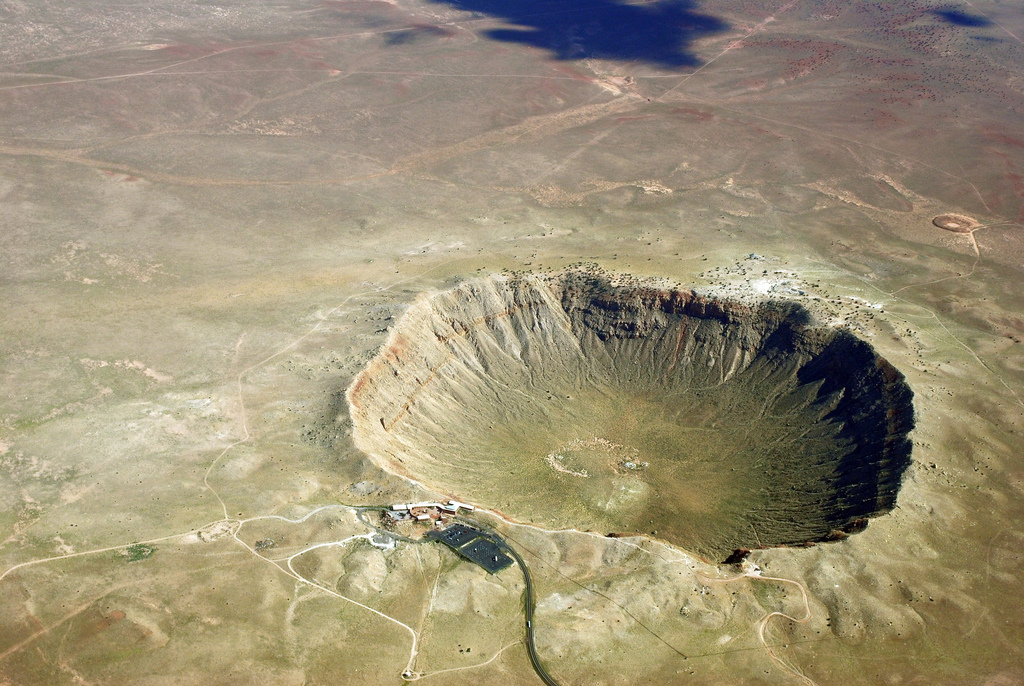
\includegraphics{meteorcrater.jpg}
\end{image}
This area was once grasslands and woodlands inhabited by bison,
camels, wooly mammoths, and giant ground sloths. During the
Pleistocene epoch, a meteor only $40$ meters in diameter collided
with the Earth and this changed very quickly. The collision released
around $4\times10^{16}$ joules of energy, comparable to the energy
released by a large nuclear weapon. A fireball extended out $10$
kilometers from the center of the impact, destroying all life in its
wake. It is estimated it took one-hundred years for the local plant
and animal life to repopulate the area.  Fifty-thousand years later,
the remains of the impact crater are still intact on our ever-changing
Earth.

To help us understand events like these, we need to precisely describe
what we are observing (in this case, the crater).  To do this we use a
\textit{contour map}, often called a \textit{topographical map}:
%% Based on Meteor Crater USGS Topographic Map
\begin{image}[2in]
\begin{tikzpicture}[y=0.80pt, x=0.80pt, yscale=-1.000000, xscale=1.000000, inner sep=0pt, outer sep=0pt]
\path[draw=black,even odd rule] (308.0482,210.3114) -- (266.7601,199.6668) --
  (248.6965,201.6022) -- (236.1165,199.9894) -- (221.9237,199.6668) --
  (212.2468,201.6022) -- (190.3125,203.8602) -- (176.4423,213.2145) --
  (164.8300,225.7945) -- (158.0561,237.7293) -- (152.2500,249.9868) --
  (149.6695,263.2119) -- (151.2823,270.6308) -- (149.3469,281.9206) --
  (150.3146,293.2103) -- (149.9921,301.9195) -- (154.1854,305.7903) --
  (153.8628,313.8543) -- (156.4433,321.2733) -- (161.2818,327.5633) --
  (170.9587,339.0143) -- (170.3136,344.1753) -- (175.4746,349.0138) --
  (180.3130,348.0461) -- (183.5387,351.2717) -- (183.5387,355.7876) --
  (188.3771,355.7876) -- (192.5704,359.6584) -- (192.2479,363.5291) --
  (198.3766,363.2066) -- (200.9571,367.0773) -- (205.7955,369.3353) --
  (207.0858,374.4963) -- (212.5694,376.4317) -- (213.5371,381.5927) --
  (223.2140,385.9473) -- (233.6973,385.7860) -- (246.7611,395.6242) --
  (256.1155,396.1081) -- (258.0508,400.9465) -- (272.8888,400.3014) --
  (282.5657,400.7852) -- (295.1457,398.0434) -- (304.6613,397.5596) --
  (319.0154,391.2696) -- (328.3697,381.5927) -- (333.2082,379.9799) --
  (339.3369,370.6255) -- (339.6594,363.8517) -- (351.9168,343.2076) --
  (352.8845,326.7569) -- (355.7876,320.6282) -- (360.6261,303.5323) --
  (363.2066,289.6621) -- (360.6261,286.4364) -- (359.9809,277.4047) --
  (362.8840,273.5339) -- (358.0455,263.5344) .. controls (358.0455,263.5344) and
  (349.6589,254.5027) .. (349.3363,251.2770) .. controls (349.0138,248.0514) and
  (346.4333,241.9227) .. (346.4333,241.9227) -- (341.5948,236.4391) --
  (339.3369,230.6329) -- (332.8856,223.2140) -- (330.9502,221.6012) --
  (328.3697,220.7948) -- (317.8864,211.7630) -- cycle;
\path[draw=black,even odd rule] (124.8321,258.6960) -- (123.5418,281.2754) --
  (126.1223,302.2421) -- (129.9931,315.1446) -- (134.1864,324.8215) --
  (133.8639,330.6277) -- (135.7993,336.4338) -- (137.7346,341.9174) --
  (144.5085,351.2717) -- (152.8951,361.9163) -- (153.2177,369.0127) --
  (160.3141,375.7866) -- (159.6690,381.5927) -- (165.7977,383.5281) --
  (173.8618,395.7855) -- (182.2484,400.3014) -- (190.9576,410.9460) --
  (199.3443,413.2039) -- (203.5376,418.0424) -- (217.0853,420.9454) --
  (227.7299,425.4613) -- (229.0201,427.3967) -- (235.1488,425.4613) --
  (302.8872,420.3003) -- (324.1764,414.4942) -- (337.7241,408.6880) --
  (343.5302,406.7527) -- (347.7235,399.0111) -- (358.6907,387.3988) --
  (362.8840,385.4635) -- (364.8194,378.6896) -- (369.9804,373.2060) --
  (374.4963,373.2060) -- (379.9799,363.8517) -- (376.7542,359.0132) --
  (381.2701,350.9492) -- (384.4958,341.5948) -- (390.9470,337.7241) --
  (389.9793,328.0471) -- (387.3988,321.2733) -- (389.0117,304.5000) --
  (386.7537,300.3067) -- (388.0440,296.1134) -- (390.9470,291.9200) --
  (389.9793,288.6944) -- (385.1409,281.9206) -- (385.1409,276.1144) --
  (379.0122,271.2760) -- (380.9476,254.1801) -- (376.1091,248.0514) --
  (376.7542,240.3099) -- (372.8835,236.1165) -- (373.5286,229.0201) --
  (369.9804,223.8591) -- (365.7871,224.1817) -- (360.3035,216.1176) --
  (359.9809,214.1822) -- (354.8199,209.9889) -- (352.2394,206.1181) --
  (346.4333,204.8279) -- (340.6271,194.5058) -- (332.2405,192.2479) --
  (325.4666,188.6997) -- (322.5636,188.3771) -- (320.6282,183.5387) --
  (309.3385,182.8935) -- (307.4031,180.9582) -- (299.6616,181.2807) --
  (295.3069,176.9261) -- (286.7590,177.4100) -- (278.0498,177.0874) --
  (271.9211,179.0228) -- (265.1473,177.0874) -- (258.3734,177.7325) --
  (249.0191,178.0551) -- (242.5678,176.7648) -- (239.0196,179.6679) --
  (223.8591,179.0228) -- (218.0530,180.9582) -- (201.6022,184.1838) --
  (182.2484,188.0546) -- (164.5074,194.8284) -- (156.1208,196.4412) --
  (153.2177,200.6345) -- (145.7987,207.7309) -- (131.6059,226.4396) --
  (130.3157,241.4388) -- (127.7352,245.9547) -- cycle;
\path[draw=black,even odd rule] (135.3154,191.4415) -- (144.3915,186.6855) --
  (147.4730,180.1045) -- (170.9587,176.7648) -- (190.3125,173.2166) --
  (203.8602,167.7331) -- (224.1817,165.1525) -- (245.7934,159.3464) .. controls
  (245.7934,159.3464) and (254.1801,161.9269) .. (257.0832,160.9592) .. controls
  (259.9862,159.9915) and (266.7601,158.7013) .. (266.7601,158.7013) .. controls
  (266.7601,158.7013) and (276.4370,160.9592) .. (278.3724,160.9592) --
  (292.2426,160.9592) .. controls (294.1780,160.9592) and (299.3390,158.7013) ..
  (301.5969,161.2818) .. controls (303.8549,163.8623) and (306.4354,166.7654) ..
  (306.4354,166.7654) -- (317.4025,165.4751) .. controls (317.4025,165.4751) and
  (324.1764,165.4751) .. (325.4666,166.4428) .. controls (326.7569,167.4105) and
  (339.9820,176.4423) .. (339.9820,176.4423) -- (345.4656,179.0228) --
  (350.6266,178.0551) -- (357.7230,188.3771) -- (367.0773,194.5058) --
  (368.0450,199.0217) -- (374.4963,203.2150) -- (376.1091,209.3438) --
  (385.4635,214.1822) -- (386.1086,218.0530) -- (392.8824,227.0848) --
  (392.8824,238.6970) -- (401.9142,260.9539) -- (405.7850,269.3406) --
  (405.1398,282.5657) -- (408.3655,295.7908) -- (408.3655,299.9841) --
  (406.7527,344.1753) -- (407.7203,350.6266) -- (398.0434,356.7553) --
  (395.7855,370.3030) -- (388.0440,375.1414) -- (387.7214,384.1732) --
  (380.6250,387.0763) -- (359.6584,406.4301) -- (357.7230,417.0747) --
  (350.9492,421.9131) -- (326.1118,423.5260) -- (314.1769,431.2675) --
  (306.1128,431.5900) -- (297.0810,435.4608) -- (232.8909,441.2670) --
  (227.4073,442.2346) -- (221.9237,447.3957) -- (215.1499,441.5895) --
  (208.3761,439.9767) -- (188.6997,431.9126) -- (180.9582,433.2029) --
  (174.5069,429.6547) -- (173.5392,416.4296) -- (169.6684,411.9137) --
  (160.6366,411.9137) -- (160.6366,406.4301) -- (150.9597,397.3983) --
  (141.2828,396.7532) -- (142.2505,388.6891) -- (139.3475,386.4311) --
  (139.6700,381.9153) -- (137.4121,378.0445) -- (134.5090,374.4963) --
  (125.4772,357.4004) -- (124.1870,351.9168) -- (116.4455,344.4979) --
  (117.0906,338.0466) -- (114.9433,328.8259) -- (112.0794,315.6008) --
  (108.7039,305.7903) -- (109.9942,300.3067) -- (107.0911,289.9846) --
  (107.0911,279.0175) -- (106.7685,267.4052) -- (104.8332,264.5021) --
  (106.1234,245.4709) -- (109.6716,241.2775) -- (109.3491,229.9878) --
  (115.4778,225.7945) -- (115.1552,219.0207) -- (120.6388,212.2468) --
  (120.9613,206.7632) -- (135.7993,190.7963);
\path[draw=black,even odd rule] (92.8983,240.3099) -- (90.9629,250.3093) -- (89.6727,271.9211)
  -- (91.9306,285.7913) -- (94.5111,295.1457) -- (96.4465,296.4359) --
  (94.8337,309.9836) -- (100.3173,320.3056) -- (100.6398,328.6923) --
  (104.8332,334.4984) -- (102.5752,340.3046) -- (106.7685,351.2717) --
  (111.6070,356.4327) -- (111.2844,363.2066) -- (119.3485,373.8512) --
  (119.6711,381.2701) -- (130.3157,388.3665) -- (131.6059,392.5599) --
  (132.5736,394.8178) -- (132.8962,401.2691) -- (139.3475,409.6557) --
  (147.7341,411.5911) -- (147.7341,418.6875) -- (158.7013,424.1711) --
  (162.2495,425.7839) -- (160.3141,431.9126) -- (177.7325,449.3310) --
  (187.0869,445.7828) -- (197.7315,447.0731) -- (212.5694,458.0403) --
  (225.7945,461.9110) -- (232.5683,456.1049) -- (243.5355,452.5567) --
  (256.1155,453.2018) -- (259.6637,450.2987) -- (272.2436,450.9439) --
  (285.1462,450.9439) -- (297.0810,447.3957) -- (310.6287,437.7188) --
  (321.2733,432.8803) -- (347.0784,432.8803) -- (362.5614,428.0418) --
  (371.2707,427.0742) -- (372.8835,416.1070) -- (382.8829,404.1721) --
  (393.2050,392.8824) -- (400.3014,380.6250) -- (405.4624,377.3994) --
  (408.0429,370.6255) -- (417.7198,358.0456) -- (418.3649,333.8533) --
  (417.0747,306.4354) -- (418.3649,296.4359) -- (415.4619,288.0493) --
  (415.4619,270.9534) -- (405.7850,241.2775) -- (404.1721,235.1488) --
  (403.2044,225.1494) -- (392.2373,209.0212) -- (380.6250,197.7315) --
  (372.8835,183.5387) -- (355.7876,167.7331) -- (345.4656,165.4751) --
  (325.7892,154.5079) -- (304.8226,153.5403) -- (297.4036,145.7987) --
  (252.5673,151.6049) -- (232.2458,149.0244) -- (206.4407,154.8305) --
  (189.9899,166.1202) -- (165.4751,172.5715) -- (143.8633,167.7331) --
  (137.0895,177.7325) -- (118.7034,191.6028) -- (113.5424,199.9894) --
  (108.0588,207.4084) -- (103.5429,211.6017) -- cycle;
\path[draw=black,even odd rule] (94.7701,206.1986) -- (94.4280,217.1467) -- (87.1292,224.9017)
  -- (84.0500,237.9026) -- (78.0057,249.8772) -- (76.0670,259.7990) --
  (79.7164,268.3522) -- (80.0585,297.3193) -- (83.9360,304.9602) --
  (83.5938,313.6275) -- (94.6561,345.5597) -- (94.1999,355.2534) --
  (99.5599,367.5700) -- (108.5694,377.1497) -- (108.2272,385.9310) --
  (119.5175,397.5635) -- (122.0265,402.5814) -- (122.5967,409.7661) --
  (127.9567,413.5295) -- (158.4063,442.2685) -- (162.8540,448.4268) --
  (162.7400,451.0498) -- (171.0652,458.4627) -- (178.0218,460.6295) --
  (186.0048,457.5503) -- (193.8738,457.2082) -- (200.6024,459.3750) --
  (205.8484,465.1912) -- (210.7523,471.9198) -- (228.6571,470.4372) --
  (243.4827,462.2261) -- (269.8268,461.0857) -- (274.0464,459.4891) --
  (282.7137,459.9452) -- (287.5035,455.3835) -- (290.5827,455.4975) --
  (291.9512,457.7784) -- (296.6270,457.7784) -- (305.4083,447.5145) --
  (311.6807,445.9179) -- (319.3216,441.4702) -- (344.4112,442.1544) --
  (352.3942,445.5757) -- (360.9475,444.8915) -- (367.4480,440.6719) --
  (371.6676,440.6719) -- (377.4838,437.1365) -- (382.1596,429.0394) --
  (382.0455,416.2666) -- (387.0634,414.8981) -- (392.8796,406.9150) --
  (396.7571,406.3448) -- (400.9767,402.0112) .. controls (400.9767,402.0112) and
  (400.5206,400.5286) .. (401.0908,400.1865) .. controls (401.6610,399.8443) and
  (403.4857,399.1601) .. (403.4857,399.1601) .. controls (403.4857,399.1601) and
  (405.5385,394.2562) .. (405.7666,393.8000) .. controls (405.9946,393.3438) and
  (406.1087,389.3523) .. (406.1087,389.3523) -- (420.7062,372.3599) --
  (421.2765,369.0526) -- (425.9522,365.7453) -- (429.3735,359.4729) --
  (429.4876,347.9546) -- (427.2067,342.5945) -- (428.6893,338.7170) --
  (430.6280,334.4974) -- (428.9174,321.1544) -- (424.6978,310.0921) --
  (425.8382,298.8018) -- (426.4084,291.5031) -- (424.2416,287.2834) --
  (423.3292,275.9931) -- (416.7147,258.4305) -- (417.9692,246.1138) --
  (413.2934,242.2363) -- (411.1266,223.9894) -- (401.5469,204.6020) --
  (393.6780,199.8121) -- (383.6421,188.0657) -- (381.3613,179.3984) --
  (371.5535,171.0732) -- (369.5007,164.2306) -- (363.0003,158.0722) --
  (347.2623,155.9054) -- (336.8843,146.4398) -- (314.8739,143.4747) --
  (306.7768,139.3691) -- (293.6619,140.0534) -- (288.9861,135.9478) --
  (259.1067,136.2899) -- (256.0275,134.1231) -- (250.3253,135.3776) --
  (244.8513,137.3163) -- (228.6571,139.4832) -- (217.1387,143.9308) --
  (210.6220,146.5882) -- (201.4952,148.2206) -- (188.4551,159.3058) --
  (172.2886,158.5189) -- (160.4591,159.1573) -- (138.9049,151.8585) --
  (132.0623,155.1071) -- (130.0095,163.4323) -- (133.3168,174.9507) .. controls
  (133.3168,174.9507) and (129.3253,178.1439) .. (128.7550,178.1439) .. controls
  (128.1848,178.1439) and (121.2282,184.8724) .. (121.2282,184.8724) --
  (117.0086,186.1269) -- (105.7183,194.1100) -- (103.3234,199.5840) -- cycle;
\path[draw=black,even odd rule] (179.8292,113.3811) .. controls (179.8292,113.3811) and
  (182.6516,105.5589) .. (182.6516,105.0751) .. controls (182.6516,104.5912) and
  (181.1194,89.9146) .. (181.1194,89.9146) -- (170.0716,83.3827) --
  (166.9266,82.2537) -- (164.3461,86.8502) -- (156.1208,94.4305) --
  (120.1549,114.8326) -- (118.0583,117.8970) -- (118.0583,124.6708) --
  (111.1231,125.9611) -- (106.9298,127.8965) .. controls (106.9298,127.8965) and
  (104.1880,125.9611) .. (103.3816,126.1223) .. controls (102.5752,126.2836) and
  (101.9301,128.7029) .. (101.9301,128.7029) -- (104.3493,132.5736) --
  (102.4139,135.6380) -- (88.3824,136.2831) .. controls (88.3824,136.2831) and
  (82.2537,129.3480) .. (81.6086,129.3480) .. controls (80.9635,129.3480) and
  (72.8994,128.8641) .. (72.8994,128.8641) -- (70.3189,135.7993) --
  (72.5768,146.2826) -- (75.3186,151.7661) .. controls (75.3186,151.7661) and
  (73.8671,154.3467) .. (73.7058,153.7015) .. controls (73.5445,153.0564) and
  (57.9002,140.9603) .. (57.9002,140.9603) .. controls (57.9002,140.9603) and
  (54.8358,146.4438) .. (54.8358,147.2503) .. controls (54.8358,148.0567) and
  (53.3843,151.6049) .. (52.7391,151.6049) .. controls (52.0940,151.6049) and
  (46.2879,151.1210) .. (44.9976,151.1210) .. controls (43.7074,151.1210) and
  (38.2238,153.0564) .. (38.2238,153.0564) -- (35.8046,167.4105) --
  (39.3528,172.0877) -- (37.4174,178.2164) -- (29.0307,182.2484) --
  (26.1276,187.2482) -- (18.7087,197.8927) -- (24.6761,204.3440) --
  (17.7410,210.3114) -- (19.0312,215.9563) -- (20.6441,220.4722) --
  (28.5469,224.5042) -- (32.7402,232.2458) -- (36.6110,239.9873) --
  (38.5463,245.7934) -- (35.4820,251.1157) -- (29.6758,252.4060) --
  (29.6758,256.7606) -- (22.4182,267.8890) -- (24.3535,275.9531) --
  (23.3859,291.9200) -- (22.9020,295.1457) -- (18.0636,310.3061) --
  (21.2892,318.6928) -- (28.2243,321.7572) -- (32.0951,321.7572) --
  (29.6758,333.8533) -- (29.8371,338.2079) -- (22.2569,338.2079) --
  (19.8377,344.4979) -- (29.3533,364.9807) -- (28.2243,376.4317) --
  (34.9981,385.4635) -- (42.2558,392.2373) -- (41.9333,397.8822) --
  (29.8371,400.3014) -- (29.0307,416.4296) -- (30.1597,429.8159) --
  (39.9979,442.3959) -- (42.4171,449.9762) -- (56.2873,468.2010) --
  (55.8035,470.6202) -- (49.3522,476.2651) -- (38.2238,476.4264) --
  (29.3533,466.5882) -- (23.5471,466.7495) -- (26.4502,472.0718) --
  (24.1923,482.2325) -- (24.5148,488.2000) -- (35.3207,496.7479) --
  (49.8361,497.2317) -- (52.7391,501.1025) -- (51.6102,508.5215) --
  (47.2556,511.7471) .. controls (47.2556,511.7471) and (47.4168,514.1663) ..
  (48.0620,514.0050) .. controls (48.7071,513.8438) and (54.8358,513.1986) ..
  (54.8358,513.1986) .. controls (54.8358,513.1986) and (63.8676,506.4248) ..
  (64.5127,506.4248) .. controls (65.1578,506.4248) and (67.4158,509.0053) ..
  (67.4158,509.0053) -- (65.6417,529.9719) -- (68.2222,533.1976) --
  (89.6727,527.5527) -- (94.5111,532.3912) -- (95.8014,535.9394) --
  (90.9629,543.0358) -- (75.6412,542.8745) -- (68.2222,552.0675) --
  (66.7707,574.4857) -- (69.6737,578.8403) -- (90.8016,580.1306) --
  (94.1886,582.7111) -- (97.2529,583.1949) -- (100.8011,590.4526) --
  (106.7685,590.2913) -- (119.9936,583.1949) -- (121.6065,583.5175) --
  (128.8641,574.9695) -- (133.8639,575.1308) -- (135.7993,577.8726) --
  (141.1216,575.2921) -- (139.0249,568.3570) -- (129.8318,557.0673) --
  (131.4446,550.7773) -- (134.6703,549.0032) -- (155.4756,548.3581) .. controls
  (155.4756,548.3581) and (162.8946,546.2614) .. (163.8623,546.1001) .. controls
  (164.8300,545.9388) and (175.6359,544.1647) .. (177.0874,544.0034) .. controls
  (178.5389,543.8422) and (190.9576,543.5196) .. (190.9576,543.5196) --
  (197.5702,542.2293) -- (203.2150,541.9068) -- (207.0858,548.6806) --
  (212.8919,551.2611) -- (219.3432,553.1965) -- (233.0522,561.7444) --
  (242.5678,563.5185) -- (248.0514,560.7768) -- (251.5996,560.4542) --
  (245.1483,570.9375) -- (245.3096,573.5180) -- (250.1480,574.9695) --
  (264.9860,574.3244) -- (267.2439,571.7439) -- (272.5662,574.1631) --
  (274.6629,574.4857) -- (274.1790,567.5506) -- (273.6952,563.3573) --
  (278.6949,553.5191) -- (277.2434,546.7452) -- (284.3398,542.7132) --
  (282.8882,537.8747) -- (293.0490,536.4232) -- (299.8228,525.9399) --
  (302.0808,521.4240) -- (339.9820,508.6827) -- (346.1107,508.8440) --
  (352.5620,502.7153) -- (364.9807,503.8443) -- (380.7863,490.1353) --
  (382.3991,488.3612) -- (410.6234,480.7810) -- (427.2354,476.9102) --
  (436.2672,468.6848) -- (436.4285,456.2661) -- (445.7828,448.2021) .. controls
  (445.7828,448.2021) and (447.8795,440.1380) .. (448.3633,439.4928) .. controls
  (448.8472,438.8477) and (462.7174,423.0421) .. (462.7174,423.0421) --
  (464.8141,410.3008) -- (467.2333,395.3016) -- (468.5236,384.0119) --
  (475.2974,379.0122) -- (486.4259,378.0445) -- (491.9094,371.5932) --
  (499.0058,370.4642) -- (495.2964,359.4971) .. controls (495.2964,359.4971) and
  (491.7482,359.4971) .. (490.7805,359.6584) .. controls (489.8128,359.8196) and
  (481.9100,361.4325) .. (481.1036,361.2712) .. controls (480.2971,361.1099) and
  (477.5554,354.1748) .. (477.5554,354.1748) .. controls (477.5554,354.1748) and
  (479.6520,350.1427) .. (479.8133,348.8525) .. controls (479.9746,347.5622) and
  (480.9423,343.0463) .. (480.9423,343.0463) -- (485.9420,338.5304) --
  (482.2325,331.9179) -- (474.3297,316.7574) -- (473.2007,302.7259) --
  (471.4266,301.1131) -- (466.5882,301.5969) -- (458.0403,290.1459) --
  (461.2659,283.2108) -- (461.5885,273.8565) -- (451.1051,256.9219) --
  (454.9759,245.7934) -- (450.9439,234.0199) -- (451.4277,220.9560) --
  (442.5572,212.2468) -- (436.7511,210.4727) -- (431.7513,200.1507) --
  (431.1062,189.1835) -- (421.1067,180.7969) -- (417.8811,167.0879) --
  (412.8814,155.6369) -- (406.2688,149.3469) -- (396.7532,138.8636) --
  (394.4952,130.4770) -- (383.3668,119.1872) -- (381.4314,113.8649) --
  (379.1735,99.9947) -- (372.0771,97.0916) -- (368.2063,100.9624) --
  (356.4327,100.8011) -- (355.6263,94.9950) -- (360.9486,88.5437) --
  (360.1422,84.3504) -- (350.7879,83.0601) -- (350.9492,77.7378) --
  (344.1753,69.1899) -- (343.2076,67.2545) -- (335.4661,71.7704) --
  (332.0792,76.7701) -- (326.5956,76.7701) -- (318.5315,85.1568) --
  (315.9510,83.2214) -- (315.1446,75.8024) -- (307.2418,70.8027) --
  (304.1774,79.3506) -- (300.3067,82.7376) -- (289.1782,83.3827) --
  (283.6947,79.6732) -- (281.9206,83.3827) -- (284.0172,87.8986) --
  (279.6626,89.1888) -- (268.8567,87.5760) -- (261.7603,96.1239) --
  (257.8896,95.6401) -- (257.4057,84.5117) -- (251.1157,76.9314) --
  (248.8578,71.4478) -- (245.9547,72.7381) -- (245.1483,80.6409) --
  (239.9873,86.6083) -- (239.0196,95.8014) -- (242.4065,101.9301) --
  (243.8580,106.2847) -- (239.3422,110.8006) -- (220.3109,109.6716) --
  (214.5048,115.1552) -- (207.5696,115.1552) -- (192.7317,123.2193) --
  (186.6030,121.1226) -- cycle;
\end{tikzpicture}
\end{image}
In essence we are looking at the crater from directly above, and each
curve in the maps above represents a fixed, constant height.
Mathematically, a contour map describes a \textit{function} of two
variables. We will now define a more general case of a function of $n$
variables. These are often called \textit{functions of several
  variables}.

\begin{definition}
  Let $D$ be a subset of $\R^n$.  A \dfn{function $F$ of several
    variables} with \dfn{domain} $D$ is a relation that assigns to
  every ordered tuple in $D$ a unique real number in $\R^n$.  We
  denote this by:

  \begin{align*}
    F: D &\to \R\\
    \vec{x} &\mapsto y\\
    \vector{x_1,x_2,\dots,x_n} &\mapsto y
  \end{align*}
  
  The \dfn{range} of $F$ is the set of all outputs of $F$.  It is a
  subset of $\R$, not $\R^n$.
\end{definition}

\begin{example}
  Consider:
  \begin{align*}
    F: \R^2 &\to \R\\
    (x,y) &\mapsto x^2+y^2
  \end{align*}
  Find the domain and range of $F$.
  \begin{explanation}
    Here, the domain is \wordChoice{\choice{$(-\infty,\infty)$}\choice[correct]{$\R^2$}\choice{$\R^n$}}
    and the range is \wordChoice{\choice{$(-\infty,\infty)$}\choice[correct]{$[0,\infty)$}\choice{$\R^2$}\choice{$\R^n$}}.
  \end{explanation}
\end{example}
The relationship from the previous example can be described more
succinctly by the equation:
\[
F(x,y)=x^2+y^2,
\]
which is the notation that we will use more frequently from here on
when describing functions.

\begin{remark}
  In this text, we will use an upper-case letter to denote a function
  of several variables.
\end{remark}

\begin{remark}
  Often times, we will not specify the domain of a function in order to
  shorten its description.  Unless otherwise specified, we will take the
  domain of a given function on $\R^n$ to be the set of all ordered
  pairs in $\R^n$ for which the function is defined.  In the above
  example, we would write $F(x,y) = x^2+y^2$, and from this, the reader
  should be able to determine the domain.
\end{remark}

Let's investigate a few functions of two variables, $F:\R^2\to\R$:

\begin{question}
  Consider
  \[
  F(x,y) = \ln(9-x^2-y^2),
  \]
  and compute $F(2,1)$.
  \begin{prompt}
    \[
    F(2,1) = \answer{\ln(4)}
    \]
  \end{prompt}
  \begin{question}
    What is the domain of $F$?
    \begin{prompt}
      Since we have not specified the domain, we take it to be the set of all vectors $\vector{x,y}$ allowable as
      \wordChoice{\choice[correct]{inputs}\choice{outputs}} for $F$.
      Because of the logarithm, we need $\vector{x,y}$ such that:
      \begin{multipleChoice}
      \choice[correct]{$0 < 9-x^2-y^2$}
      \choice{ $ 0 \leq 9-x^2-y^2$}
      \choice{$  0 > 9-x^2-y^2$}
      \choice{ $ 0 \geq 9-x^2-y^2$}
      \end{multipleChoice}

      The observant young mathematician may note that this inequality
      describes the interior of a circle of radius $\answer[given]{3}$
      centered at $(0,0)$ in the $(x,y)$-plane since we can write:
      \begin{align*}
        0 & < 9-x^2-y^2 \\
        \answer{x^2+y^2} &< 9.
      \end{align*}
      While the domain may not always be easy to visualize, it is
      often insightful to take a step back after finding it and ask
      this question.
    \end{prompt}
    \begin{question}
      What is the range of $F$?
      \begin{prompt}
        The range is the set of all possible
        \wordChoice{\choice{input}\choice[correct]{output}} values.  The
        logarithm allows for outputs between $(-\infty,\infty)$ is there is no restriction on the size of the inputs.  In general, the logarithm is an \wordChoice{\choice[correct]{larger}\choice{smaller}} function of its input; as the input gets larger, the outputs get \wordChoice{\choice[correct]{larger}\choice{smaller}} . Since 
        the $x$ and $y$ terms are squared, then subtracted, inside the
        square-root, the largest output value comes at $x=\answer{0}$,
        $y=\answer{0}$, where $F(0,0) = \answer{\ln(9)}$.  Since the inputs can become arbitrarily close to $0$ as we approach any point on the circle $x^2+y^2=9$, the range $R$ is the interval $(\answer{-\infty},\answer{\ln(9)}]$.
      \end{prompt}
    \end{question}
  \end{question}
\end{question}

Now let's ponder functions of three variables, $F:\R^3\to\R$. Consider
this geometric example:
\begin{example}
  The volume of a cylinder with base radius $R$ and height $h$ is
  given by:
  \[
  V=\pi R^2h
  \]
  We can now think of the volume of a cylinder as a function of two
  variables, $R$ and $h$:
  \[
  V(R,h) = \pi R^2h
  \]
  Find the domain and the range of $V$.
  \begin{explanation}
    By requiring that the radius and height be nonnegative, we find that the domain is
    \wordChoice{
      \choice{$\R$}
      \choice{$[0,\infty)$}
      \choice[correct]{$\{ (R,h) \in \R^2 : R \geq 0, h \geq 0\}$}
      }. 
The range is:
\wordChoice{
  \choice{$\R$}
  \choice[correct]{$[0,\infty)$}
  \choice{$\{ (R,h) \in \R^2 : R \geq 0, h \geq 0\}$}
  }.
Here, the domain represents the set of all possible nonnegative radii and heights of the cylinder, and the range represents the set of all possible volumes that a cylinder could have.
  \end{explanation}
\end{example}




\section{Visualizing functions of several variables}

There are many ways to interpret a function of several variables.  Two
very common ways to do this are to graph the function or look at
``level sets'' of our function, which we define shortly.

Recall that given a function $f(x)$ of a single variable, we can
consider the equation $y=f(x)$, which allows us to visualize the
function as the set of all points $(x,y)$ in the $(x,y)$-plane.  To do
this, we pick an $x$-value in the domain, and then the corresponding
$y$-coordinate is given by $F(x)$.

%Include graph?%

Given a function $F(x,y)$ of two variables, we can take the same
approach.  We'll consider the set of all points in the $(x,y,z)$-space
where $z=F(x,y)$.  By choosing a point $(x,y)$ in the domain of the
function, the corresponding $z$-coordinate will be given by $F(x,y)$:
\begin{image}
  \begin{tikzpicture}
    \begin{axis}[tick label style={font=\scriptsize},axis on top,
	axis lines=center,
	view={110}{25},
	name=myplot,
	xtick=\empty,
        ytick=\empty,
        ztick=\empty,
	ymin=-.1,ymax=1.2,
	xmin=-.1,xmax=1.2,
	zmin=-.2, zmax=2.1,
	every axis x label/.style={at={(axis cs:\pgfkeysvalueof{/pgfplots/xmax},0,0)},xshift=-1pt,yshift=-4pt},
	xlabel={\scriptsize $x$},
	every axis y label/.style={at={(axis cs:0,\pgfkeysvalueof{/pgfplots/ymax},0)},xshift=5pt,yshift=-3pt},
	ylabel={\scriptsize $y$},
	every axis z label/.style={at={(axis cs:0,0,\pgfkeysvalueof{/pgfplots/zmax})},xshift=0pt,yshift=4pt},
	zlabel={\scriptsize $z$},
        colormap/cool,
      ]
      \addplot3[gray,domain=0:2,samples y=0,dashed] ({1*cos(45)},{1*sin(45)},x); %% line for z
      \addplot3[gray,domain=0:cos(45),samples y=0,dashed] ({x},{1*sin(45)},0); %% line for x
      \addplot3[gray,domain=0:cos(45),samples y=0,dashed] ({sin(45)},{x},0); %% line for y
      \filldraw [black] (axis cs:{1*cos(45)},{1*sin(45)},1.95) circle (2.5pt);        
      \node[right] at (axis cs:{1*cos(45)},{1*sin(45)},2) {$(x,y,F(x,y))$};

      \filldraw [black!50!white] (axis cs:{1*cos(45)},{1*sin(45)},0) circle (2.5pt);        
      \node[below right,black!50!white] at (axis cs:{1*cos(45)},{1*sin(45)},0) {$(x,y)$};
    \end{axis}
  \end{tikzpicture}
\end{image}

Thus, one way of visualizing the function $F(x,y)$ is to consider the
equation $z=F(x,y)$ and interpret that the function assigns a
``height'' to each point $(x,y)$ in its domain.

To make a sketch of a surface, we can specify many locations in the
$(x,y)$-plane (by picking many different values for $x$ and $y$), and
plot the corresponding heights.  While this is tedious to do by hand,
computers can do it very easily.  For example, if we consider the
function $F(x,y) = 2-4x^3+y^2$, we can evaluate the function at many
different $(x,y)$ and plot the results.  For instance, at the point
$(x,y)=(1,2)$, we have $F(1,2) = \answer[given]{2}$.  Using software
to graph both the surface and this point gives:

\begin{image}
  \begin{tikzpicture}
    \begin{axis}[tick label style={font=\scriptsize},axis on top,
	axis lines=center,
	view={110}{25},
	name=myplot,
	xtick=\empty,
        ytick=\empty,
        ztick=\empty,
	ymin=-.25,ymax=2.2,
	xmin=-.25,xmax=2.2,
	zmin=-.5, zmax=5.1,
	every axis x label/.style={at={(axis cs:\pgfkeysvalueof{/pgfplots/xmax},0,0)},xshift=-1pt,yshift=-4pt},
	xlabel={\scriptsize $x$},
	every axis y label/.style={at={(axis cs:0,\pgfkeysvalueof{/pgfplots/ymax},0)},xshift=5pt,yshift=-3pt},
	ylabel={\scriptsize $y$},
	every axis z label/.style={at={(axis cs:0,0,\pgfkeysvalueof{/pgfplots/zmax})},xshift=0pt,yshift=4pt},
	zlabel={\scriptsize $z$},
        colormap/cool,
      ]
      \addplot3[gray,domain=0:2,samples y=0,dashed] ({1*cos(45)},{1*sin(45)},x); %% line for z
      \addplot3[gray,domain=0:cos(45),samples y=0,dashed] ({x},{1*sin(45)},0); %% line for x
      \addplot3[gray,domain=0:cos(45),samples y=0,dashed] ({sin(45)},{x},0); %% line for y
\addplot3[domain=-.3:2.2,y domain=-.3:2.5,mesh,samples y=25,very thin,z buffer=sort,  samples=25,] (x,y,{2-4*x^3+y^2});            
      \filldraw [black] (axis cs:{1*cos(45)},{1*sin(45)},1.95) circle (2.5pt);        
      \node[right] at (axis cs:{1*cos(45)},{1*sin(45)},1.9) {$(1,2,2)$};

      \filldraw [black!50!white] (axis cs:{1*cos(45)},{1*sin(45)},0) circle (2.5pt);        
      \node[below right,black!50!white] at (axis cs:{1*cos(45)},{1*sin(45)},0) {$(1,2)$};
    \end{axis}
  \end{tikzpicture}
\end{image}

\begin{remark}
In general, given a function $F: \R^n \to \R$, we can set $x_{n+1} =
F(x_1, x_2,\dots , x_n)$ and generalize the idea above.  In this case
though, we cannot represent the graph of the function as we did
before.
\end{remark}

This now allows us to present a concept that will play a pivotal role
in much of this course.

\subsection{Curves on surfaces}

Recall that a curve in $\R^n$ is simply a collection of points in
$\R^n$ where the coordinates of any point on the curve can be
determined from a single parameter.  Specializing to functions $F:\R^2
\to \R$, where we can provide good visual examples, note that we can
consider curves that lie in the domain of $F$.  We can evaluate
$F(x,y)$ at each point on this curve in the $(x,y)$-plane, and doing this
allows us to plot these points on the surface.

\begin{example}
To see this in action, consider the earlier example $F(x,y) = 2-x^3+y^2$ and consider the curve defined by $y=2x$ in the $(x,y)$-plane.  Note that the domain of $F(x,y) = 2-x^3+y^2$ is all of $\R^2$, so each point that lies along $y=2x$ also is in the domain of $F$.

Fill out the table below:

\[\begin{array}{c|c|c}
x & y =2x & z=2-x^3+y^2\\
\hline
-0.5 & \answer[given]{-1} & \answer[given]{3.5}\\
0 & \answer[given]{0} & \answer[given]{2}\\
0.5 & \answer[given]{1} &  \answer[given]{2.5}\\
1 & \answer[given]{2} & \answer[given]{2}\\
\end{array}\]

We can plot each of these points $(x,y)$ on the line $y=2x$ in the $(x,y)$-plane, then plot the corresponding points $(x,y,F(x,y))$ on the surface.  In fact, we can do this at \emph{every} point on the line $y=2x$ to plot the curve that lies on the surface directly above (or below) this line:

\begin{image}
  \begin{tikzpicture}
    \begin{axis}[tick label style={font=\scriptsize},axis on top,
	axis lines=center,
	view={110}{25},
	name=myplot,
	xtick=\empty,
        ytick=\empty,
        ztick=\empty,
	ymin=-.8,ymax=2.2,
	xmin=-.8,xmax=2.2,
	zmin=-.5, zmax=5.1,
	every axis x label/.style={at={(axis cs:\pgfkeysvalueof{/pgfplots/xmax},0,0)},xshift=-1pt,yshift=-4pt},
	xlabel={\scriptsize $x$},
	every axis y label/.style={at={(axis cs:0,\pgfkeysvalueof{/pgfplots/ymax},0)},xshift=5pt,yshift=-3pt},
	ylabel={\scriptsize $y$},
	every axis z label/.style={at={(axis cs:0,0,\pgfkeysvalueof{/pgfplots/zmax})},xshift=0pt,yshift=4pt},
	zlabel={\scriptsize $z$},
        colormap/cool,
      ]
%      \addplot3[gray,domain=0:2,samples y=0,dashed] ({1*cos(45)},{1*sin(45)},x); %% line for z
%      \addplot3[gray,domain=0:cos(45),samples y=0,dashed] ({x},{1*sin(45)},0); %% line for x
%      \addplot3[gray,domain=0:cos(45),samples y=0,dashed] ({sin(45)},{x},0); %% line for y
\addplot3[domain=-.8:2.2,y domain=-.8:2.5,mesh,samples y=25,very thin,z buffer=sort,  samples=25,] (x,y,{2-4*x^3+y^2});   
\addplot3 [very thick,penColor, smooth,domain=-.39:3,samples=20,samples y=0] ({x},{2*x},{2-4*x^3+4*x^2});
\addplot3 [very thick,penColor, dashed,domain=-.5:3,samples=20,samples y=0] ({x},{2*x},{0});
     

%points they plotted in the xy plane and point on curve%
	%\node[below,black!50!white] at (axis cs:{-.5*cos(45)},{-1*sin(45)},0) {$(-.5,-1)$};
		      \filldraw [black] (axis cs:{-.5*cos(45)},{-1*sin(45)},0) circle (2.5pt); 
		      \filldraw [black] (axis cs:{-.5*cos(45)},{-1*sin(45)},2.6768) circle (2.5pt);  
	       	      \addplot3[black,thick, domain=0:2.6768,samples y=0,dashed] ({-.5*cos(45)},{-1*sin(45)},x); %% line for z 
      	%\node[below,black!50!white] at (axis cs:{0*cos(45)},{0*sin(45)},0) {$(0,0)$};
		  \filldraw [black] (axis cs:{0*cos(45)},{0*sin(45)},0) circle (2.5pt); 
		  \filldraw [black] (axis cs:{0*cos(45)},{0*sin(45)},2) circle (2.5pt);  
		  \addplot3[black,thick, domain=0:2,samples y=0,dashed] ({0*cos(45)},{0*sin(45)},x); %% line for z 
      	%\node[below,black!50!white] at (axis cs:{.5*cos(45)},{1*sin(45)},0) {$(.5,1)$};
		  \filldraw [black] (axis cs:{.5*cos(45)},{1*sin(45)},0) circle (2.5pt); 
		  \filldraw [black] (axis cs:{.5*cos(45)},{1*sin(45)},2.3232) circle (2.5pt); 
		  \addplot3[black,thick, domain=0:2.3232,samples y=0,dashed] ({.5*cos(45)},{1*sin(45)},x); %% line for z  
      	%\node[below,black!50!white] at (axis cs:{1*cos(45)},{2*sin(45)},0) {$(1,2)$};
	  	\filldraw [black] (axis cs:{1*cos(45)},{2*sin(45)},0) circle (2.5pt); 
		\filldraw [black] (axis cs:{1*cos(45)},{2*sin(45)},2.5858) circle (2.5pt);  
		\addplot3[black,thick, domain=0:2.5858,samples y=0,dashed] ({1*cos(45)},{2*sin(45)},x); %% line for z 
      	%\node[below,black!50!white] at (axis cs:{1.5*cos(45)},{3*sin(45)},0) {$(1.5,3)$};
	  	\filldraw [black] (axis cs:{1.5*cos(45)},{3*sin(45)},0) circle (2.5pt); 
		\filldraw [black] (axis cs:{1.5*cos(45)},{3*sin(45)},1.727) circle (2.5pt);
		\addplot3[black,thick, domain=0:1.727,samples y=0,dashed] ({1.5*cos(45)},{3*sin(45)},x); %% line for z   		

    \end{axis}
  \end{tikzpicture}
  
  %%%%%SHOULD WE LABEL THESE POINTS?%%%%%%%%%
\end{image}

\end{example} 

Take a second back and think what we just did before we continue.  We
can naturally visualize that a function $F(x,y)$ associates a
``height'' to each point in its domain.  Since curves are collections
of points, the function assigns a height to each point along a curve
in its domain.  In this way, the function can be thought to ``lift'' a
curve in its domain onto the surface $z=F(x,y)$ in $(x,y,z)$-space.

While this hopefully is not too taxing to think about conceptually, the question now arises: How do we actually give a description of the curve on the surface above a curve in the domain of the function?  For curves in the $(x,y)$-plane, we can describe a curve by:

\begin{itemize}
\item Giving $x$ as an explicit function of $y$.
\item Giving $y$ as an explicit function of $x$.
\item Giving a description of $x$ and $y$ in terms of a parameter $t$.
\end{itemize}

While the latter is used mostly when we have a dynamic situation in
mind in the $(x,y)$-plane, it must be used almost out of necessity to
give descriptions of curves in $\R^3$.  Until now, most of the
parameterized curves in $\R^3$ were given to you, but we are now in a
position to construct our own. For an explicit example, let's return
to the function in the previous example.

\begin{example}
  Let $F(x,y) = 2-x^3+y^2$ and suppose we want to give a parametric
  description of the the curve that lies on this surface above the line
  $y=2x$ in the $(x,y)$-plane.
  \begin{explanation}
    In order to do this, we should first parameterize the curve in the
    $(x,y)$-plane.  Since $y$ is an explicit function of $x$, we
    choose $x(t)=t$, and thus $y(t)=\answer[given]{2t}$.  We can now
    use the surface, which relates $z$ to $x$ and $y$, and our
    parameterization to find $z$ in terms of $t$.  In fact, since
    $z=2-x^3+y^2$, setting $x=t$ and expressing $y$ in terms of $t$
    gives $z(t) = \answer[given]{2+4t^2-t^3}$. Thus, a
    parameterization of the curve is:
    \[
    \vec{p}(t) =\vector{\answer[given]{t} , \answer[given]{2t}, \answer[given]{2+4t^2-t^3}}
    \]
  \end{explanation}
\end{example}

\begin{remark}
We are going to get substantial mileage out of thinking about curves
on the surface that lie above curves in the domain.  Indeed, this will
arise when we discuss limits of functions of several variables,
derivatives and differentiability, chain rule, tangent planes, and
constrained optimization later in this chapter.  It is important that
you get a good intuitive feel for this conceptually as well as make
sure you remember whether we are considering curves in the domain, for
example the $(x,y)$-plane, or curves on the surface, for example
$(x,y,z)$-space.
\end{remark}

\section{Level sets}

It was Descartes who said ``\link[Je pense, donc je
  suis]{https://en.wikipedia.org/wiki/Cogito,_ergo_sum},'' He also
developed our rectangular coordinate system, the $(x,y)$-plane. This
is also known as the \link[Cartesian coordinate
  system]{https://en.wikipedia.org/wiki/Cartesian_coordinate_system}.
This coordinate system allows us to consider the graph of the
function. First, recall that the graph of a function of a single
variable, $y=f(x)$ is a curve in a two-dimensional plane.  In the same
sense, the graph of a function of two variables, $z = F(x,y)$ is a
surface in three-dimensional space. The graph of a function of three
variables, $w=F(x,y,z)$ is a surface in \textit{four}-dimensional
space. A surfaces in higher than three dimensions is often called a
\dfn{hypersuface}. How can we visualize such functions?  For
visualizing functions $f:\R\to\R$, a graphing utility like
\link[\textsl{Desmos}]{https://www.desmos.com/} is really great. For
visualizing functions $F:\R^2\to\R$,
\link[\textsl{GeoGebra}]{https://www.geogebra.org/3d} is very
helpful. However, once we get to functions $F:\R^3\to\R$, we can no
longer visualize the graph of the function as we did before.  One
powerful technique to help us understand a function $F:\R^3\to\R$
visually is know as sketching \textit{level sets}.


\begin{definition}
  Suppose that $F:\R^n \to \R$ is a function and $c$ is in the range
  of $F$. A \dfn{level set} corresponding to $F(\vec{x})=c$ is a set
  in the domain of the function such that $F(\vec{x}) = c$ for all
  points in the set.
\end{definition}

%% \begin{remark}
%% Some people call the curve on the surface $z=F(x,y)$ that lies
%% directly above (or below) the level curve a \dfn{contour curve}.
%% \end{remark}


It may be surprising to find that the concept of level sets is
familiar to most people (they just don't realize it).  Topographical
maps, like the one below represent the surface of Earth by
indicating points with the same elevation with \dfn{contour
  lines}.

\begin{image}%%Allegheny College: http://sitesmedia.s3.amazonaws.com/creekconnections/files/2014/09/topomap.jpg
  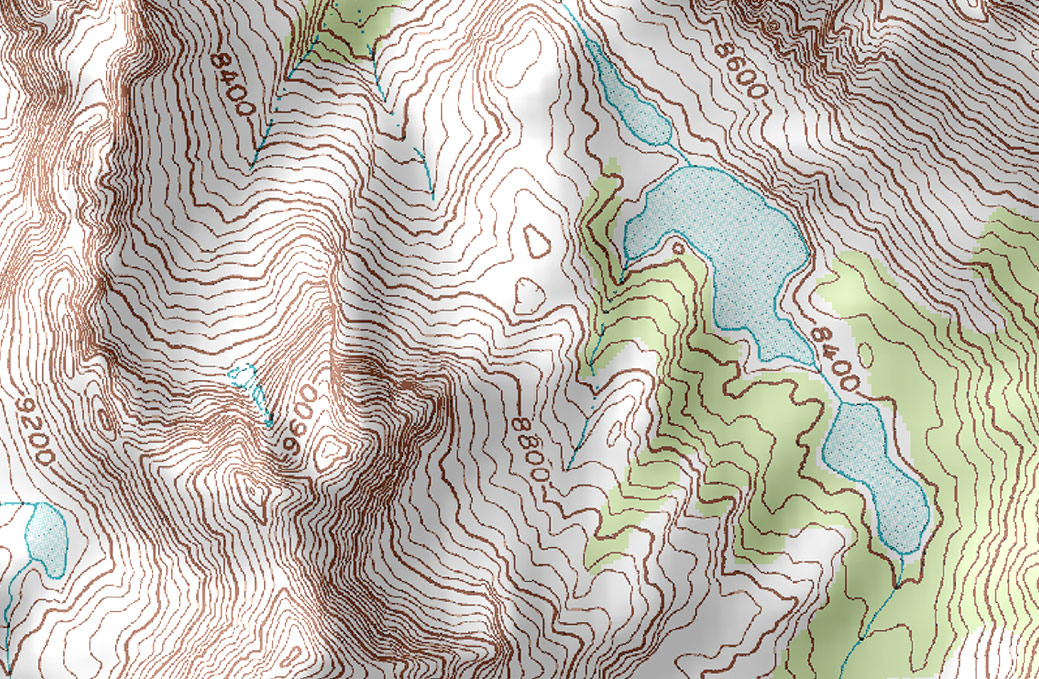
\includegraphics{topomap.jpg}
\end{image}

Another example you may know are \dfn{isotherms}, curves where the
temperatures are the same. We see these in weather maps:

\begin{image}
  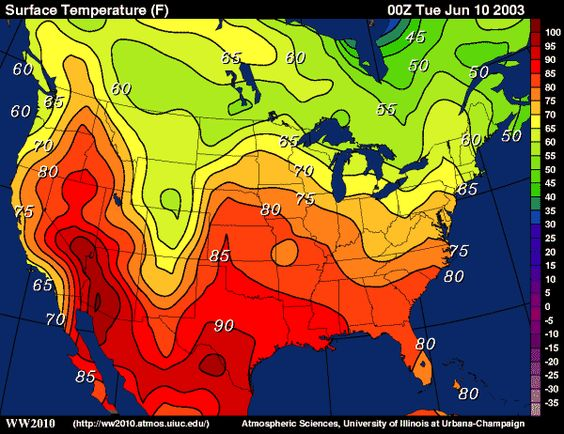
\includegraphics{isotherm.jpg}
\end{image}

When working with functions $F:\R^2\to\R$ the level sets are known as
\dfn{level curves}.  Below we see a surface with level curves drawn
beneath the surface:

\begin{image}
  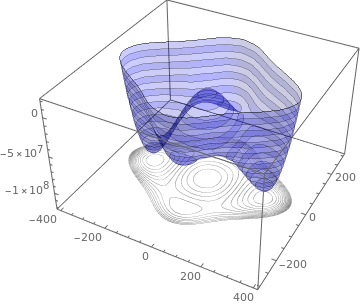
\includegraphics{firstContourPlot.png}
\end{image}

%% \begin{question} BADBAD Bart would like to add a question here
%%   Matching level curves to surfaces.
%% \end{question}

If the ``heights'' of the level curves are equally spaced, then level
curves are close together when the function is changing rapidly, and
far apart when the function is changing slowly.

\begin{question}
  \begin{image}
    \begin{tikzpicture}	
      \draw[very thick, penColor] plot[smooth cycle] coordinates{(10,4) (9,3) (10,3)};
      \draw[very thick, penColor] plot[smooth cycle] coordinates{(11,2) (10,5) (8,3)};
      \draw[very thick, penColor] plot[smooth cycle] coordinates{
        (7,3) (12,1) (10,6) (7,5) (5,6) (5,5) (7,4)
      };
      \draw[very thick, penColor] plot[smooth cycle] coordinates{
        (13,0) (10,7) (4,9) (1,8) (1,4) (5,1)
      };

%        \node[penColor,fill=white] at (axis cs:2,2.66) {$7$};
    \end{tikzpicture}
  \end{image}
\end{question}


\subsection{Working with level curves}

Let's work within the scenario for functions $F:\R^2 \to \R$ since
they are easier to visualize.  The idea behind a level set is fairly
intuitive.  Rather than picking points along a grid in the
$(x,y)$-plane and evaluating the function at these points, we can pick
a $z$-value, say $z=c$, in the range of the function and ask ``at
which points $(x,y)$ can we evaluate the function to get $F(x,y)=c$?''
Those points form our level set.  Before moving on, take a second to
try to visualize what we just described for a function $z=F(x,y)$.
\begin{example}
  Given that $z=c$ is in the range of $z=F(x,y)$, select the
  statements below that are true:
  \begin{selectAll}
    \choice[correct]{The level curves $F(x,y)=c$ are curves in the domain of the function.} 
    \choice[correct]{The level curves $F(x,y)=c$ are curves in the $(x,y)$-plane.} 
    \choice{The level curves $F(x,y)=c$ are curves in the range of the function.} 
    \choice{The level curves $F(x,y)=c$ are curves on the surface $z=F(x,y)$.} 
    \choice{The level curves $F(x,y)=c$ can also be thought of as the intersection of the plane $z=c$ with the surface $z=F(x,y)$.} 
  \end{selectAll}
\end{example}


\begin{remark}
  If we choose a value $z=c$ that was not in the range of $F$, there
  would be no points in the $(x,y)$-plane for which $F(x,y)=c$, and
  hence no level curve associated to it.
\end{remark}



Now it's time for an example.

\begin{example}
  Suppose that $F(x,y) = \sqrt{1-\frac{x^2}{9}-\frac{y^2}{4}}$.  Find
  the domain and range of $F$ and sketch the level curves for for
  $c=0$, $0.2$, $0.4$, $0.6$, $0.8$ and $1$.
  \begin{explanation}
    The domain of $F$ is
    \wordChoice{
      \choice{$\R$}
      \choice{$\R^2$}
      \choice{$\{ (x,y) \in \R^2 :1-\frac{x^2}{9}-\frac{y^2}{4} >0 \}$}
      \choice[correct]{$\{ (x,y) \in \R^2 :1-\frac{x^2}{9}-\frac{y^2}{4} \geq0 \}$}
      }. 
    The range of $F$ is
    \wordChoice{
      \choice{$\R$}
      \choice{$\R^2$}
      \choice{$[0,\infty)$}
      \choice[correct]{$[0,1]$}
      }.

      Now let's find the level curves of $F$ for $c=0$, $0.2$, $0.4$,
      $0.6$, $0.8$ and $1$ (note that each of these $c$-values is in
      the range of $F$). Each of our level curves will be of the form
      \begin{align*}
        c &= \sqrt{1-\frac{x^2}{9}-\frac{y^2}{4}}\\
        c^2 &= \answer[given]{1-\frac{x^2}{9}-\frac{y^2}{4}}.
      \end{align*}
      Now we just need to substitute all of our values for $c$ and
      plot each of the following implicit functions:
    \begin{align*}
      0^2   &= 1-\frac{x^2}{9}-\frac{y^2}{4}, \\
      0.2^2 &= 1-\frac{x^2}{9}-\frac{y^2}{4}, \\
      0.4^2 &= 1-\frac{x^2}{9}-\frac{y^2}{4}, \\
      0.6^2 &= 1-\frac{x^2}{9}-\frac{y^2}{4}, \\
      0.8^2 &= 1-\frac{x^2}{9}-\frac{y^2}{4}, \\
        1^2 &= 1-\frac{x^2}{9}-\frac{y^2}{4}.   
    \end{align*}
    You can now plot these implicit functions with your favorite
    graphing device, or recognize that they are ellipses.
    \begin{onlineOnly}
      As a gesture of friendship, we have included a graph of these
      level curves:
      \[
      \graph[xmin=-5, xmax=5, ymin=-2.3, ymax=2.3]{0^2 = 1-\frac{x^2}{9}-\frac{y^2}{4}, 0.2^2 = 1-\frac{x^2}{9}-\frac{y^2}{4}, 0.4^2 = 1-\frac{x^2}{9}-\frac{y^2}{4},0.6^2 = 1-\frac{x^2}{9}-\frac{y^2}{4},0.8^2 = 1-\frac{x^2}{9}-\frac{y^2}{4},1^2 = 1-\frac{x^2}{9}-\frac{y^2}{4}}
      \]
    \end{onlineOnly}
    In the image below, the level curves are drawn on a graph of $F$
    in space.
    \begin{image}
      \begin{tikzpicture}
        \begin{axis}%
          [tick label style={font=\scriptsize},axis on top,
	    axis lines=center,
	    view={135}{25},
	    name=myplot,
	    %xtick=\empty,
	    %ytick=\empty,
	    %ztick=\empty,
	    ymin=-3.1,ymax=3.1,
	    xmin=-3.1,xmax=3.1,
	    zmin=-.1, zmax=2.1,
	    every axis x label/.style={at={(axis cs:\pgfkeysvalueof{/pgfplots/xmax},0,0)},xshift=-3pt,yshift=-3pt},
	    xlabel={\scriptsize $x$},
	    every axis y label/.style={at={(axis cs:0,\pgfkeysvalueof{/pgfplots/ymax},0)},xshift=5pt,yshift=-2pt},
	    ylabel={\scriptsize $y$},
	    every axis z label/.style={at={(axis cs:0,0,\pgfkeysvalueof{/pgfplots/zmax})},xshift=0pt,yshift=4pt},
	    zlabel={\scriptsize $z$},colormap/cool
	  ]
          \addplot3[domain=0:180,mesh,y domain=0:180,samples y=30,very thin,z buffer=sort,samples=30,] ({3*cos(x)*cos(y)},{2*sin(x)*cos(y)},{sin(y)});
          
          \addplot3 [very thick,penColor, smooth,domain=-40:170,samples=60,samples y=0] ({3*(cos(x))},{2*(sin(x))},0);

          \addplot3 [very thick,penColor, smooth,domain=-40:170,samples=60,samples y=0] ({2.93*(cos(x))},{1.96*(sin(x))},.2);
          
          \addplot3 [very thick,penColor, smooth,domain=-40:170,samples=60,samples y=0] ({2.75*(cos(x))},{1.83*(sin(x))},.4);
          
          \addplot3 [very thick,penColor, smooth,domain=-40:170,samples=60,samples y=0] ({2.4*(cos(x))},{1.6*(sin(x))},.6);
          
          \addplot3 [very thick,penColor, smooth,domain=-40:170,samples=60,samples y=0] ({1.8*(cos(x))},{1.2*(sin(x))},.8);
          
          %\filldraw [penColor] (axis cs: 0,0,1) circle (1pt);          
        \end{axis}
      \end{tikzpicture}
    \end{image}
    Note how the elevations are evenly spaced. Near the
    level curves of $c=0$ and $c=0.2$ we can see that $F$ indeed is
    growing quickly.
  \end{explanation}
\end{example}



\begin{example}
  Suppose that $F(x,y) = x^2-y^2$. Find
  the domain and range of $F$ and sketch the level curves for for
  $c=-3$, $-2$, $-1$, $0$, $1$, $2$, and $3$.
  \begin{explanation}
    The domain of $F$ is
    \wordChoice{
      \choice{$\R$}
      \choice[correct]{$\R^2$}
      \choice{$\{ (x,y) \in \R^2 :1-\frac{x^2}{9}-\frac{y^2}{4} >0 \}$}
      \choice{$\{ (x,y) \in \R^2 :1-\frac{x^2}{9}-\frac{y^2}{4} \geq0 \}$}
      }. 
    The range of $F$ is
    \wordChoice{
      \choice{$\R$}
      \choice[correct]{$\R^2$}
      \choice{$[0,\infty)$}
      \choice{$[0,1]$}
      }.

      Now let's find the level curves of $F$ for the required values.
      Each of our level curves will be of the form
      \[
      c = \answer[given]{x^2-y^2}
      \]
      Now we just need to substitute all of our values for $c$ and
      plot each of the following implicit functions:
    \begin{align*}
      -3 &= x^2-y^2\\
      -2 &= x^2-y^2\\
      -1 &= x^2-y^2\\
       0 &= x^2-y^2\\
       1 &= x^2-y^2\\
       2 &= x^2-y^2\\
       3 &= x^2-y^2
    \end{align*}
    You can now plot these implicit functions with your favorite
    graphing device, or recognize that they are crossing lines when
    $x=y=0$ and hyperbolas otherwise.
    \begin{onlineOnly}
      As a gesture of friendship, we have included a graph of these
      level curves:
      \[
      \graph[xmin=-5, xmax=5, ymin=-2.5, ymax=2.5]{-3=x^2-y^2,-2=x^2-y^2,-1=x^2-y^2,0=x^2-y^2,1=x^2-y^2,2=x^2-y^2,3=x^2-y^2}
      \]
    \end{onlineOnly}
    In the image below, the level curves are drawn on a graph of $F$
    in space.
    \begin{image}
      \begin{tikzpicture}
        \begin{axis}%
          [tick label style={font=\scriptsize},axis on top,
	    axis lines=center,
	    view={147}{30},
	    name=myplot,
	    %xtick=\empty,
	    %ytick=\empty,
	    %ztick=\empty,
	    ymin=-3.5,ymax=3.5,
	    xmin=-3.5,xmax=3.5,
	    zmin=-3.5, zmax=3.5,
	    every axis x label/.style={at={(axis cs:\pgfkeysvalueof{/pgfplots/xmax},0,0)},xshift=-5pt,yshift=-1pt},
            xlabel={\scriptsize $x$},
            every axis y label/.style={at={(axis cs:0,\pgfkeysvalueof{/pgfplots/ymax},0)},xshift=4pt,yshift=-4pt},
            ylabel={\scriptsize $y$},
            every axis z label/.style={at={(axis cs:0,0,\pgfkeysvalueof{/pgfplots/zmax})},xshift=0pt,yshift=4pt},
            colormap/cool
	  ]
          \addplot3[mesh,samples y=15,domain=-2:2, y domain=-2:2,very thin,z buffer=sort,samples=30,] ({x},{y},{x^2-y^2});
          
          \addplot3 [very thick,penColor,domain=-2:2,smooth,samples=60,samples y=0] ({x},{x},0);
          \addplot3 [very thick,penColor,domain=-2:2,smooth,samples=60,samples y=0] ({x},{-x},0);
          
          \addplot3 [very thick,penColor, smooth,samples=60,samples y=0,domain=-1.33:1.33] ({cosh(x)},{sinh(x)},1);
          \addplot3 [very thick,penColor, smooth,samples=60,samples y=0,domain=-1.33:1.33] ({-cosh(x)},{sinh(x)},1);

          \addplot3 [very thick,penColor, smooth,samples=60,samples y=0,domain=-.9:.9] ({sqrt(2)*cosh(x)},{sqrt(2)*sinh(x)},2);
          \addplot3 [very thick,penColor, smooth,samples=60,samples y=0,domain=-.9:.9] ({-sqrt(2)*cosh(x)},{sqrt(2)*sinh(x)},2);

          \addplot3 [very thick,penColor, smooth,samples=60,samples y=0,domain=-.55:.55] ({sqrt(3)*cosh(x)},{sqrt(3)*sinh(x)},3);
          \addplot3 [very thick,penColor, smooth,samples=60,samples y=0,domain=-.55:.55] ({-sqrt(3)*cosh(x)},{sqrt(3)*sinh(x)},3);


          \addplot3 [very thick,penColor, smooth,samples=60,samples y=0,domain=-1.33:1.33] ({sinh(x)},{cosh(x)},-1);
          \addplot3 [very thick,penColor, smooth,samples=60,samples y=0,domain=-1.33:1.33] ({sinh x)},{-cosh(x)},-1);

          \addplot3 [very thick,penColor, smooth,samples=60,samples y=0,domain=-.9:.9] ({sqrt(2)*sinh(x)},{sqrt(2)*cosh(x)},-2);
          \addplot3 [very thick,penColor, smooth,samples=60,samples y=0,domain=-.9:.9] ({sqrt(2)*sinh(x)},{-sqrt(2)*cosh(x)},-2);

          \addplot3 [very thick,penColor, smooth,samples=60,samples y=0,domain=-.55:.55] ({sqrt(3)*sinh(x)},{sqrt(3)*cosh(x)},-3);
          \addplot3 [very thick,penColor, smooth,samples=60,samples y=0,domain=-.55:.55] ({sqrt(3)*sinh(x)},{-sqrt(3)*cosh(x)},-3);
          
        \end{axis}
      \end{tikzpicture}
    \end{image}
  \end{explanation}
\end{example}




 
%% We illustrate these ideas with a picture.  Consider the function,
%% $F(x,y) = 5-4x+y^2$.  Noting that the domain of this function is
%% $\R^2$ and the range is $\R$, we can choose any value for $c$ that we
%% want.
 
%% \begin{itemize}
%% \item If we choose $c=1$, the set of all points in the domain of $F$ for which $z=0$ is found easily by setting $z= 5-4x+y^2 = 1$.  This is the curve in the $(x,y)$-plane described by $4x-y^2 = 1$ or $x= \frac{1}{4}+ \frac{1}{4}y^2$.
%% \item If we choose $c=5$, the set of all points in the domain of $F$ for which $z=0$ is found easily by setting $z= 5-4x+y^2 = 4$. This is the curve in the $(x,y)$-plane described by $4x-y^2 = 0$ or $x= \frac{1}{4}y^2$.
%% \end{itemize}

%% We now plot the level curves and the contour curves on the same plot:   
   
%% \begin{image}
%%   \begin{tikzpicture}
%%     \begin{axis}[tick label style={font=\scriptsize},axis on top,
%% 	axis lines=center,
%% 	view={110}{25},
%% 	name=myplot,
%% 	xtick=\empty,
%%         ytick=\empty,
%%         ztick=\empty,
%% 	ymin=-1,ymax=1,
%% 	xmin=-.5,xmax=1,
%% 	zmin=-.5, zmax=9,
%% 	every axis x label/.style={at={(axis cs:\pgfkeysvalueof{/pgfplots/xmax},0,0)},xshift=-1pt,yshift=-4pt},
%% 	xlabel={\scriptsize $x$},
%% 	every axis y label/.style={at={(axis cs:0,\pgfkeysvalueof{/pgfplots/ymax},0)},xshift=5pt,yshift=-3pt},
%% 	ylabel={\scriptsize $y$},
%% 	every axis z label/.style={at={(axis cs:0,0,\pgfkeysvalueof{/pgfplots/zmax})},xshift=0pt,yshift=4pt},
%% 	zlabel={\scriptsize $z$},
%%         colormap/cool,
%%       ]
%% %      \addplot3[gray,domain=0:2,samples y=0,dashed] ({1*cos(45)},{1*sin(45)},x); %% line for z
%% %      \addplot3[gray,domain=0:cos(45),samples y=0,dashed] ({x},{1*sin(45)},0); %% line for x
%% %      \addplot3[gray,domain=0:cos(45),samples y=0,dashed] ({sin(45)},{x},0); %% line for y
%% \addplot3[domain=-1:2,y domain=-1:2,mesh,samples y=25,very thin,z buffer=sort,  samples=25,] (x,y,{5-4*x+y^2});   
%% \addplot3 [very thick,penColor, smooth,domain=-1:2,samples=20,samples y=0] ({(.25+.25*x^2)},{x},{1});
%% \addplot3 [very thick,penColor, dashed,domain=-1:2,samples=20,samples y=0] ({(.25+.25*x^2)},{x},{0});
%% \addplot3 [very thick,penColor2, smooth,domain=-1:2,samples=20,samples y=0] ({(.25*x^2)},{x},{4});
%% \addplot3 [very thick,penColor2, dashed,domain=-1:2,samples=20,samples y=0] ({(.25*x^2)},{x},{0});
%%        \end{axis}
%%   \end{tikzpicture}
  
%%  \end{image}
 
%% \begin{center}
%%   The dashed lines represent the level curves corresponding to $z=1$ and $z=5$.  The smooth lines on the surface represent the contour curves on the surface.  Note that the contour curve associated to $z=1$ can be found by ``lifting'' the corresponding level curve up $1$ unit, while the contour curve associated to $z=5$ can be found by ``lifting'' the corresponding level curve up $5$ units.
%% \end{center}

 
%%%%%%%%%%%%%%%%%%%%%%%%%%%%%%%%%%%%%%%%%%%%%%%%%%%% 


Try your hand at these questions:


\begin{question}
Suppose that $F(x,y) = 4xy+3y^2+3$.  

Are there any values of $c$ where there is no level curve associated to $z=c$?
\begin{multipleChoice}
\choice{Yes; the domain of $F$ is not all of $\R^2$}
\choice{No; the domain of $F$ is all of $\R^2$}
\choice{Yes; the range of $F$ is not all of $\R$}
\choice[correct]{No; the range of $F$ is all of $\R$}
\end{multipleChoice}

\begin{question}
Find the equation of the level curve that passes through $(x,y) = (1,2)$ in terms of $x$ and $y$.

\begin{prompt}
The level curve consists of all points in the $(x,y)$-plane that give the same value for $F(x,y)$.  Since $(1,2)$ lies on this curve, and $F(1,2) = \answer[given]{23}$, the equation of the level curve is $4xy+3y^2+3 = \answer[given]{23}$, or $4xy+3y^2 = \answer[given]{20}$ 
\end{prompt}

\begin{question}
Give a parametric description for both the level curve and the
corresponding curve on the surface.

\begin{prompt}
Since the level curve is given by the equation $4xy+3y^2 = 20$ and we
can solve for $x$ without too much algebra, we set $y=t$.  Then, $x
=\answer[given]{\frac{5}{t}-\frac{3}{4}t^2}$.

The level curve can be described parametrically by:
\[
\vec{p} (t) = \vector{\answer[given]{\frac{5}{t}-\frac{3}{4}t^2}, t}
\]
and the corresponding curve on the surface can be described
parametrically by:

\[
\vec{q} (t) = \vector{\answer[given]{\frac{5}{t}-\frac{3}{4}t^2}, t, \answer{23}}
\]

\begin{feedback}
Note that the $z$-component of the curve on the surface should not
require much calculation; we found the curve on the surface by noting
$F(1,2) =23$, so all of the $z$-values on the curve on the surface
should be $23$.
\end{feedback}

\end{prompt}

\end{question}
\end{question}
\end{question}  
  
So far the level sets we've been working with have been curves in
$\R^2$. We can easily generalize to functions $F:\R^n \to \R$.  When
working with functions $F:\R^3\to\R$, our level sets are \textit{level
  surfaces}.  \index{level sets}



%%%@BART: For the second example, I think you had mentioned something about quadric surfaces.  I've commented out what is below this for you to typeset such an example.%%%%%

%If one example is good, two is better.
%
%\begin{example}
%  Let $F(x,y) = \frac{x+y}{x^2+y^2+1}$. Find the level curves for $z=c$.
%  \begin{explanation}
%    We begin by setting $F(x,y)=c$ for an arbitrary $c$ and seeing if
%    algebraic manipulation of the equation reveals anything
%    significant.
%    \begin{align*}
%      \frac{x+y}{x^2+y^2+1} &= c \\
%      x+y &= \answer[given]{c(x^2+y^2+1)}.
%    \end{align*}
%    You may recognize this as a circle; regardless, plotting
%    \[
%    x+y = c(x^2+y^2+1).
%    \]
%    for $c=0,\pm 0.2$, $\pm 0.4$, and $\pm 0.6$ will reveal the shape of the
%    surface defined by $F$.
%    \begin{onlineOnly}
%      As a gesture of friendship, we have included a graph of these
%      level curves:
%      \[
%      \graph[xmin=-15, xmax=15, ymin=-7, ymax=7]{x+y = 0.6(x^2+y^2+1),x+y = 0.4(x^2+y^2+1), x+y = 0.2(x^2+y^2+1),x+y = 0,x+y = -0.2(x^2+y^2+1),x+y = -0.4(x^2+y^2+1),x+y = -0.6(x^2+y^2+1)}
%      \]
%    \end{onlineOnly}
%    \begin{image}
%      \begin{tikzpicture}
%        \begin{axis}%
%          [tick label style={font=\scriptsize},axis on top,
%	    axis lines=center,
%	    view={30}{30},
%	    name=myplot,
%            %width=5in,
%	    %xtick=\empty,
%	    %ytick={5},
%	    %ztick={.7,-.7},
%	    ymin=-6.6,ymax=6.6,
%	    xmin=-6.6,xmax=6.6,
%	    zmin=-.8, zmax=.8,
%	    every axis x label/.style={at={(axis cs:\pgfkeysvalueof{/pgfplots/xmax},0,0)},xshift=5pt,yshift=0pt},
%	    xlabel={\scriptsize $x$},
%	    every axis y label/.style={at={(axis cs:0,\pgfkeysvalueof{/pgfplots/ymax},0)},xshift=4pt,yshift=2pt},
%	    ylabel={\scriptsize $y$},
%	    every axis z label/.style={at={(axis cs:0,0,\pgfkeysvalueof{/pgfplots/zmax})},xshift=0pt,yshift=4pt},
%	    zlabel={\scriptsize $z$},
%            colormap/cool
%	  ]
%          \addplot3[domain=-6.5:6.5,y domain=-6.5:6.5,mesh,samples y=30,very thin,z buffer=sort,
%            samples=30,] {(x+y)/(x^2+y^2+1)};
%          \addplot3 [very thick,penColor, smooth,domain=0:360,samples=60,samples y=0] ({-0.833333 + 0.62361*cos(x)},{-0.833333 + 0.62361*sin(x)},-.6);
%          \addplot3 [very thick,penColor, smooth,domain=0:360,] ({-1.25 + 1.45774*cos(x)}, {-1.25 + 1.45774*sin(x)},-.4);
%          \addplot3 [very thick,penColor, smooth,domain=0:360,] ({-2.5 + 3.39116*cos(x)},{-2.5 + 3.39116*sin(x)},-.2);
%          \addplot3 [very thick,penColor,domain=-5:5] (x,-x,0);
%          \addplot3 [very thick,penColor, smooth,domain=0:360,] ({2.5 + 3.39116*cos(x)}, {2.5 + 3.39116*sin(x)},.2);
%          \addplot3 [very thick,penColor, smooth,domain=0:360,] ({1.25 + 1.45774*cos(x)},{1.25 + 1.45774*sin(x)},.4);
%          \addplot3 [very thick,penColor, smooth,domain=0:360,] ({0.833333 + 0.62361*cos(x)},{0.833333 + 0.62361*sin(x)},.6);
%          %\filldraw [penColor] (axis cs: 0,0,1) circle (1pt);
%        \end{axis}
%      \end{tikzpicture}
%    \end{image}
%    Seeing the level curves helps us understand the graph. For
%    instance, the graph does not make it clear that one can ``walk''
%    along the line $y=-x$ without elevation change, though the level
%    curve does.
%  \end{explanation}
%\end{example}


\subsection{Working with level surfaces}
Let's summarize a few things so far:

\begin{itemize}
  \item A function of \textbf{one} variable can be visualized as a \textbf{curve} drawn
    in \textbf{two} dimensions.
  \item A function of \textbf{two} variables can be visualized as a \textbf{surface}
    drawn in \textbf{three} dimensions.
  \item A function of \textbf{three} variables can be visualized as a
    \textbf{hypersurface} drawn in \textbf{four} dimensions.
\end{itemize}

Note that it is very difficult to produce a meaningful graph of a function of
three variables.

There are a few techniques one can employ to try to ``picture'' a
graph of three variables. One is an analogue of level curves:
\dfn{level surfaces}. Given $w=F(x,y,z)$, the level surface at $w=c$
is the surface in space formed by all points $(x,y,z)$ where
$F(x,y,z)=c$. Time for an example.


\begin{example}
  If a point source $S$ is radiating energy, the intensity $I$ at a
  given point $P$ in space is inversely proportional to the square of
  the distance between $S$ and $P$. That is, when $S=(0,0,0)$,
  \begin{align*}
  I(x,y,z) &= \frac{\text{some constant}}{\text{distance squared}}\\
  &=\frac{k}{x^2+y^2+z^2}
  \end{align*}
  for some constant $k$.  Let $k=1$; find the level surfaces of $I$.
  \begin{explanation}
    We can (mostly) answer this question using ``common sense.'' If
    energy (say, in the form of light) is emanating from the origin,
    its intensity will be the same all a points equidistant from the
    origin. That is, at any point on the surface of a sphere centered
    at the origin, the intensity should be the same. Therefore, the
    level surfaces are spheres.
    
    We now confirm this ``common sense'' mathematically. The level
    surface at $I=c$ is defined by
    \[
    c = \frac{1}{x^2+y^2+z^2}.
    \]
    Algebra reveals
    \[
    \answer[given]{x^2+y^2+z^2} = \frac{1}{c}.
    \]
    Given an intensity $c$, the level surface $I=c$ is a sphere of
    radius $1/\sqrt{c}$, centered at the origin. Every point on each
    sphere experiences the same intensity of the radiating energy.
  \end{explanation}
\end{example}

\begin{question}
  In the example above, if the distance is doubled, is the intensity
  halved?
  \begin{prompt}
  \begin{multipleChoice}
    \choice{yes}
    \choice[correct]{no}
  \end{multipleChoice}
  \begin{feedback}
    Experiment with how the level surface changes when the intensity
    is halved. We can see that that the closer one is to the source,
    the more rapidly the intensity changes.
  \end{feedback}
  \end{prompt}
\end{question}


\subsection{From explicit surfaces to level surfaces}

We turn our attention to an important concept that will arise again in
future sections:

\begin{quote}
Suppose that $F:\R^2 \to \R$ is a function of two variables.  Then, the surface $z = F(x,y)$ is a level surface of the function $G(x,y,z) = F(x,y) - z.$
\end{quote}

Now, let's consider a specific example.

\begin{example}
  Suppose that $z=x^2+y-3$. Find a function $G:\R^3\to\R$ such that
  $z=x^2+y-3$ is a level surface of $G$.
  \begin{explanation}
    We can move $z$ to the right-hand side to obtain:
    \[
    0 = \answer[given]{x^2+y-3-z}
    \]
    We can now set $G(x,y,z) = x^2+y-3-z$ and recognize that our
    original surface is the level surface of $G(x,y,z) = x^2+y-3-z$
    corresponding to $G(x,y,z)=0$.
  \end{explanation}
\end{example}

A young mathematician should rightfully demand to know why we bring up
such a fact.  Indeed, all we did here was some easy algebra.  We made
a new function of one more variable by simply rearranging the original
equation that defined our surface.  What could possibly be gained from
this?  As it turns out, the content of this procedure is vital for:
\begin{itemize}
\item Finding normal vectors for explicitly defined surfaces.
\item Finding tangent planes for explicitly defined surfaces.
\end{itemize}

Both of these results will be explored further in later sections.  We
simply introduce the fact above to you now so you can become familiar
with it before seeing how it arises in other contexts.

\section{Old problems in new settings}
To end this section, note that if we have a function of $n$ variables
and a curve in its domain, we can describe the position of each point
on the curve in terms of a single parameter, say $t$.  The outputs
above this curve are given in terms of $n$ variables, each of which
can be described in terms of $t$.  This means that the values that the
function $F$ takes above the curve can be expressed in terms of a
single variable.  Since this is the case, we can ask many familiar
questions from calculus of a single variable, or interpret several old
problems in this new setting.  Here's an example:


\begin{example}
Find the maximum area of a rectangle that can be inscribed inside of the ellipse $\frac{x^2}{4}+\frac{y^2}{9} =1$.

\begin{explanation}
Consider the image below:

 \begin{image}
            \begin{tikzpicture}
            	\begin{axis}[
            		domain=-10:10, ymax=3.6,xmax=3.6, ymin=-3.6, xmin=-3.6,
            		axis lines =center, xlabel=$x$, ylabel=$y$, ytick={-3,-2,-1,1,2,3},
            		every axis y label/.style={at=(current axis.above origin),anchor=south},
            		every axis x label/.style={at=(current axis.right of origin),anchor=west},
            		axis on top,
            		]
                      

		
                 %ellipse
                  \addplot [draw=penColor,domain=-1.8:1.8,ultra thick,smooth] {sqrt(9- 9/4*x^2)};
                  \addplot [draw=penColor,domain=-2:-1.8,ultra thick,smooth,samples=200] {sqrt(9- 9/4*x^2)};
                  \addplot [draw=penColor,domain=1.8:2,ultra thick,smooth,samples=200] {sqrt(9- 9/4*x^2)};
                  \addplot [draw=penColor,domain=-1.8:1.8,ultra thick,smooth] {-sqrt(9- 9/4*x^2)};
                  \addplot [draw=penColor,domain=-2:-1.8,ultra thick,smooth,samples=200] {-sqrt(9- 9/4*x^2)};
                  \addplot [draw=penColor,domain=1.8:2,ultra thick,smooth,samples=200] {-sqrt(9- 9/4*x^2)};

               	\node at (axis cs:11,1.55) [penColor] {$\frac{x^2}{4}+\frac{y^2}{9} =1$};
            	
		%rectangle
	     	\addplot [penColor2,very thick] plot coordinates {(-1.2,-2.4) (1.2,-2.4)(1.2,2.4)(-1.2,2.4)(-1.2,-2.4)};
	
		 \addplot[color=penColor2,fill=penColor2,only marks,mark=*] coordinates{(1.2,2.4)};
		 \node at (axis cs:1.8,2.6) [penColor2] {$(x,y)$};
	    
	      \end{axis}
            \end{tikzpicture}
            \end{image}
The area of a rectangle centered at the origin whose upper right corner is in the first quadrant is:

\[
A(x,y) = 4xy
\]
\end{explanation}

We can now see that this area is a function of two variables, $x$ and $y$.  With no additional restrictions, we see that by requiring that $(x,y)$ lies in the first quadrant, the domain of $A(x,y)$ will be $\{ (x,y) \in \R^2 : x \geq 0, y \geq 0 \}$ and the range will be $\R$.  Hence, the function $z = A(x,y)$ is a surface in the $(x,y,z)$-space whose output is the area of such a rectangle to each point in its domain. 

However, we now introduce that $(x,y)$ must also lie on the ellipse $\frac{x^2}{4}+\frac{y^2}{9} =1$, which is a curve in the domain of the function.  We thus must examine the outputs of $z=A(x,y)$ along this curve.  

When you encountered an example like this before discussing parameterizations, you likely solved for one of the variables in terms of the other.  There is nothing wrong about doing this, but it leads to messy differentiation and algebra.  When dealing with circles and ellipses, it is often convenient to use knowledge of polar coordinates (and trigonometric identities) to give a nicer description.  Here, we set:

\begin{align*}
x(\theta) &= 2 \cos(\theta) \\
y(\theta) &= 3 \sin(\theta)
\end{align*}
so we can make use of the identity $\cos^2(\theta) + \sin^2(\theta) =1$.  Indeed, by substituting these results for $x$and $y$ into the left-hand side, we find:

\begin{align*}
  \frac{x^2}{4}+\frac{y^2}{9} &=\frac{(2 \cos(\theta))^2}{4}+\frac{(3 \sin(\theta))^2}{9}\\
  &=\frac{4 \cos^2(\theta)}{4}+\frac{9 \sin(\theta)^2}{9}\\
  &=1
\end{align*}
%BART: what is the cancel command?  \cancel and \cancelto don't seem to work...
We can now express the area $A(x,y)$ evaluated along the ellipse as a
function of a single variable, $\theta$:
\begin{align*}
  A &= 4xy \\
  &= 4(2 \cos(\theta) )(3 \sin(\theta) ) \\
  &= 24 \sin(\theta)\cos(\theta)
\end{align*}
Since $x$ and $y$ are nonnegative, we have $0\le \theta \le \pi/2$.  We can perform the usual analysis (find the critical points, evaluate the function at the relevant ones in $[0,\pi/2]$, check the end points, then select the maximum), or we can use the trigonometric identity $2\sin(\theta)\cos(\theta) = \sin(2\theta)$ and write:

\begin{align*}
  A(\theta) &= 24 \sin(\theta)\cos(\theta)\\
  &= 12 \sin(2 \theta)
\end{align*}

Since $\sin(2 \theta)$ is maximized when its input $2 \theta = \frac{\pi}{2}$, we find the maximum occurs when $\theta = \answer[given]{\frac{\pi}{4}}$, which is in the allowable values for $\theta$.  Since the actual maximum of  $\sin(2 \theta)$ is $1$, we find that the maximum area is: $A=12$.

(Had we been asked, we could find the $x$ and $y$ values that give
this area by using our parametric description.)
\end{example}

\begin{remark}
The above example is an example of \emph{constrained
  optimization}---when we are looking for a minimum or maximum value
of a function subject to certain conditions.  This is a fundamentally
important idea and arises in many real world applications where
companies only have so many raw materials, employees, etc.  After we
develop more tools later in this chapter, we will revisit problems
like this one - as well as more general ones - and use these tools to
introduce a new method of solving these called \emph{Lagrange
  Multipliers}.
\end{remark}


\end{document}
